\subsection{Second Experience}

\subsubsection{Using ipconfig}

After flushing the DNS cache with \texttt{ipconfig /flushdns}, we used
\texttt{ipconfig /all} to get details about our current network configuration.
We're able to see that our IP address is \textit{10.100.229.91}, our subnet
mask is \textit{255.255.224.0}, and our default gateway is
\textit{10.100.224.1}. We can also see that the DNS servers configured on our
host are \textit{10.100.2.21} and \textit{10.100.2.22}. They're assigned via
DHCP (Dynamic Host Control Protocol), as the output indicates that it is
enabled.

The output showed several network interfaces, but the only one currently in use
is the wireless one, as we're connected to the university's WiFi network.

\begin{figure}[htbp]
    \centering
    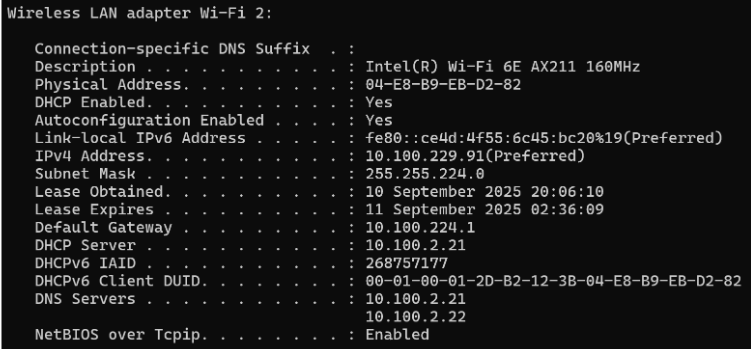
\includegraphics[width=1\linewidth]{img/9.png}
    \caption{ipconfig /all output}\label{fig:9}
\end{figure}

Before flushing the DNS cache in the initial step, there were some resource
records already stored. Most of them were related to Microsoft services, like
CDNs for updates and telemetry, like \textit{dl.delivery.mp.microsoft.com}, or
\textit{ cl-glcb907925.globalcdn.co}.

Flushing the DNS cache itself removes most records, except for the ones
mentioned just now, and some specific DNS overrides used in a previous course.
These entries map the hostnames mongo1, mongo2, and mongo3 to
\textit{127.0.0.1}, i.e.\ localhost.

\begin{figure}[htbp]
    \centering
    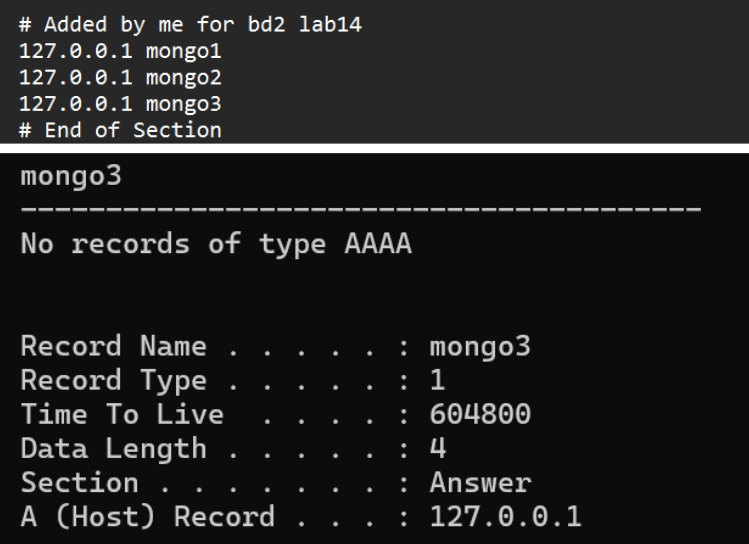
\includegraphics[width=1\linewidth]{img/10.png}
    \caption{Mongo DNS overrides}\label{fig:10}
\end{figure}

\subsubsection{DNS lookup}

With the goal of understanding server contact priority, we set nslookup type to
mail exchange (MX) and queried \textit{cisco.com}. There's three non
authoritative answers, and the server which will be contacted first is the one
with the lowest MX preference (alln-mx-01.cisco.com).

\begin{figure}[htbp]
    \centering
    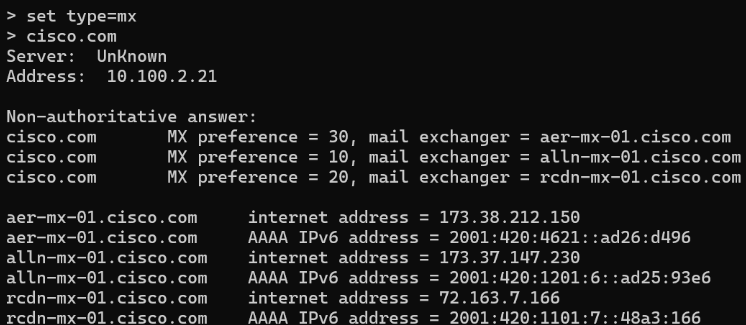
\includegraphics[width=1\linewidth]{img/11.png}
    \caption{cisco.com MX query}\label{fig:11}
\end{figure}

We then tried the same query, but this time for the hostname
\textit{gmail.com}. The first server to be contacted will be
\textit{gmail-smtp-in.l.google.com}.

\begin{figure}[htbp]
    \centering
    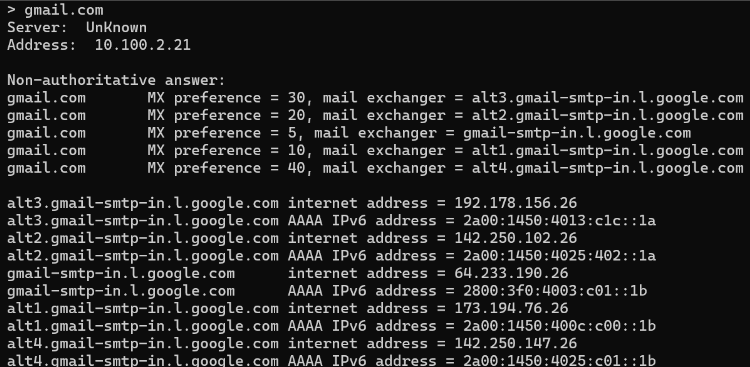
\includegraphics[width=1\linewidth]{img/12.png}
    \caption{gmail.com MX query}\label{fig:12}
\end{figure}

Finally, we used \texttt{ipconfig /all} one more time to see the DNS servers
used by the university, which are \textit{10.100.2.21} and
\textit{10.100.2.22}.

\begin{figure}[htbp]
    \centering
    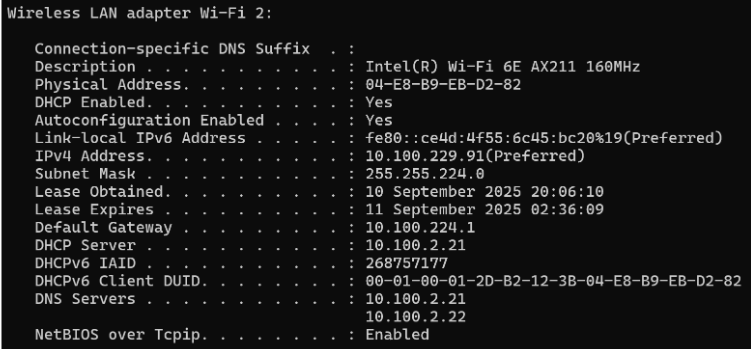
\includegraphics[width=1\linewidth]{img/9.png}
    \caption{ipconfig /all output}\label{fig:9_repeated}
\end{figure}